\documentclass[tikz,border=5pt]{standalone}
\usepackage{amsmath}
\usetikzlibrary{arrows.meta,calc}
\definecolor{ink}{HTML}{16324F}
\definecolor{teal}{HTML}{168A88}
\definecolor{gold}{HTML}{D9892B}
\definecolor{redq}{HTML}{B84A4A}
\begin{document}
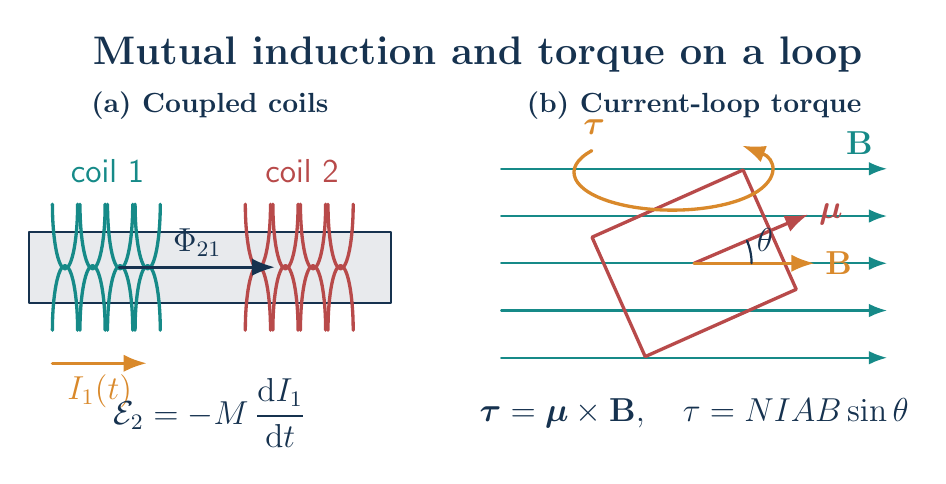
\begin{tikzpicture}[font=\large\sffamily,>=Latex,line cap=round,line join=round]
  \node[font=\bfseries\Large,ink] at (6.15,5.05)
    {Mutual induction and torque on a loop};

  \begin{scope}[shift={(.2,.45)}]
    \node[font=\bfseries,ink] at (2.55,3.95) {(a) Coupled coils};
    \fill[ink!10] (.25,1.45) rectangle (4.85,2.35);
    \draw[ink,thick] (.25,1.45) rectangle (4.85,2.35);
    \foreach \x in {.55,.9,1.25,1.60}{
      \draw[teal,very thick] (\x,1.1) arc[start angle=180,end angle=0,x radius=.16,y radius=.82];
      \draw[teal,very thick] (\x+.32,2.7) arc[start angle=0,end angle=-180,x radius=.16,y radius=.82];
    }
    \foreach \x in {3.0,3.35,3.70,4.05}{
      \draw[redq,very thick] (\x,1.1) arc[start angle=180,end angle=0,x radius=.16,y radius=.82];
      \draw[redq,very thick] (\x+.32,2.7) arc[start angle=0,end angle=-180,x radius=.16,y radius=.82];
    }
    \node[teal] at (1.25,3.12) {coil 1};
    \node[redq] at (3.72,3.12) {coil 2};
    \draw[->,ink,very thick] (1.4,1.9)--(3.38,1.9) node[midway,above] {$\Phi_{21}$};
    \draw[->,gold,very thick] (.55,.68)--(1.75,.68) node[midway,below] {$I_1(t)$};
    \node[ink] at (2.55,.05)
      {$\displaystyle \mathcal E_2=-M\,\frac{\mathrm dI_1}{\mathrm dt}$};
  \end{scope}

  \begin{scope}[shift={(6.35,.45)}]
    \node[font=\bfseries,ink] at (2.55,3.95) {(b) Current-loop torque};
    \foreach \y in {.75,1.35,1.95,2.55,3.15}
      \draw[->,teal,thick] (.1,\y)--(5.0,\y);
    \node[teal] at (4.65,3.48) {$\mathbf B$};
    \draw[redq,very thick,rotate around={24:(2.55,1.95)}]
      (1.5,1.12) rectangle (3.6,2.78);
    \draw[->,redq,very thick] (2.55,1.95)--(4.0,2.57) node[right] {$\boldsymbol\mu$};
    \draw[->,gold,very thick] (2.55,1.95)--(4.08,1.95) node[right] {$\mathbf B$};
    \draw[ink,thick] (3.28,1.95) arc[start angle=0,end angle=23,radius=.73];
    \node[ink] at (3.45,2.25) {$\theta$};
    \draw[->,gold,very thick] (1.25,3.38)
      arc[start angle=145,end angle=405,x radius=1.25,y radius=.48];
    \node[gold] at (1.28,3.68) {$\boldsymbol\tau$};
    \node[ink] at (2.55,.05)
      {$\displaystyle \boldsymbol\tau=\boldsymbol\mu\times\mathbf B,\quad
        \tau=NIAB\sin\theta$};
  \end{scope}
\end{tikzpicture}
\end{document}
